\chapter{First episodes failures}
\label{chap:reward_structure}
\begin{quotation}
\noindent ``\emph{quote}''
\begin{flushright}\textbf{author}\end{flushright}
\end{quotation}

Let us now look at why the reward of the first episode in a dual-episode
trial drops to random policy level when we know the agent is able to receive
an almost perfect reward in a single-episode trial. To understand why, we will
keep the same setting as previously (see Section~\ref{section:setting}), but
we will vary the length (in number of episodes) of the trials.

\section{Training for more episodes}
There is a recurrent pattern visible in Figure~\ref{fig:20permsLR_training}.
Indeed, no matter the number of episodes in each trial, the last one will
always reach optimal or near-optimal performance while all previous episodes
will receive a reward which corresponds to following a random policy.\\

This is confirmed by the plots of Figure~\ref{fig:20permsLR_rewards} which
show the rewards obtained by playing several trials of 2, 5 and 10 episodes
(after having trained on trials of corresponding length) over all the
permutations of the training set. Only the last episode of the trial will
succeed or almost succeed.

\begin{figure}
	\centering
	\subfloat[][Training over 1 episode]{
		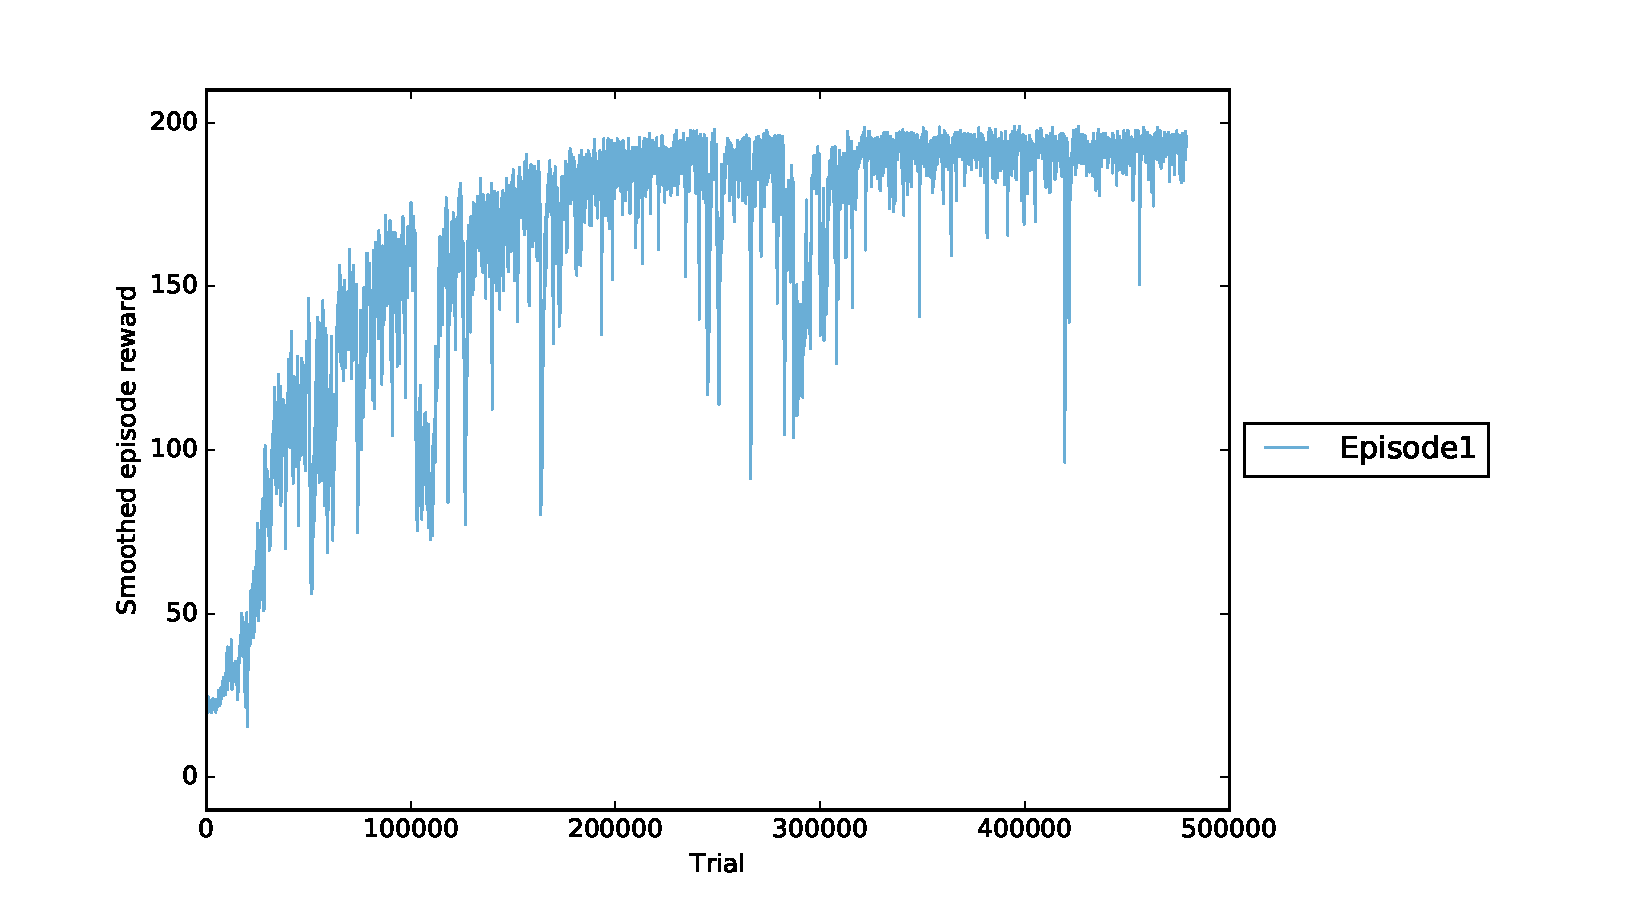
\includegraphics[width=0.49\linewidth]{fig/20permsLR1ep_training.pdf}}
	\subfloat[][Training over 2 episodes]{
		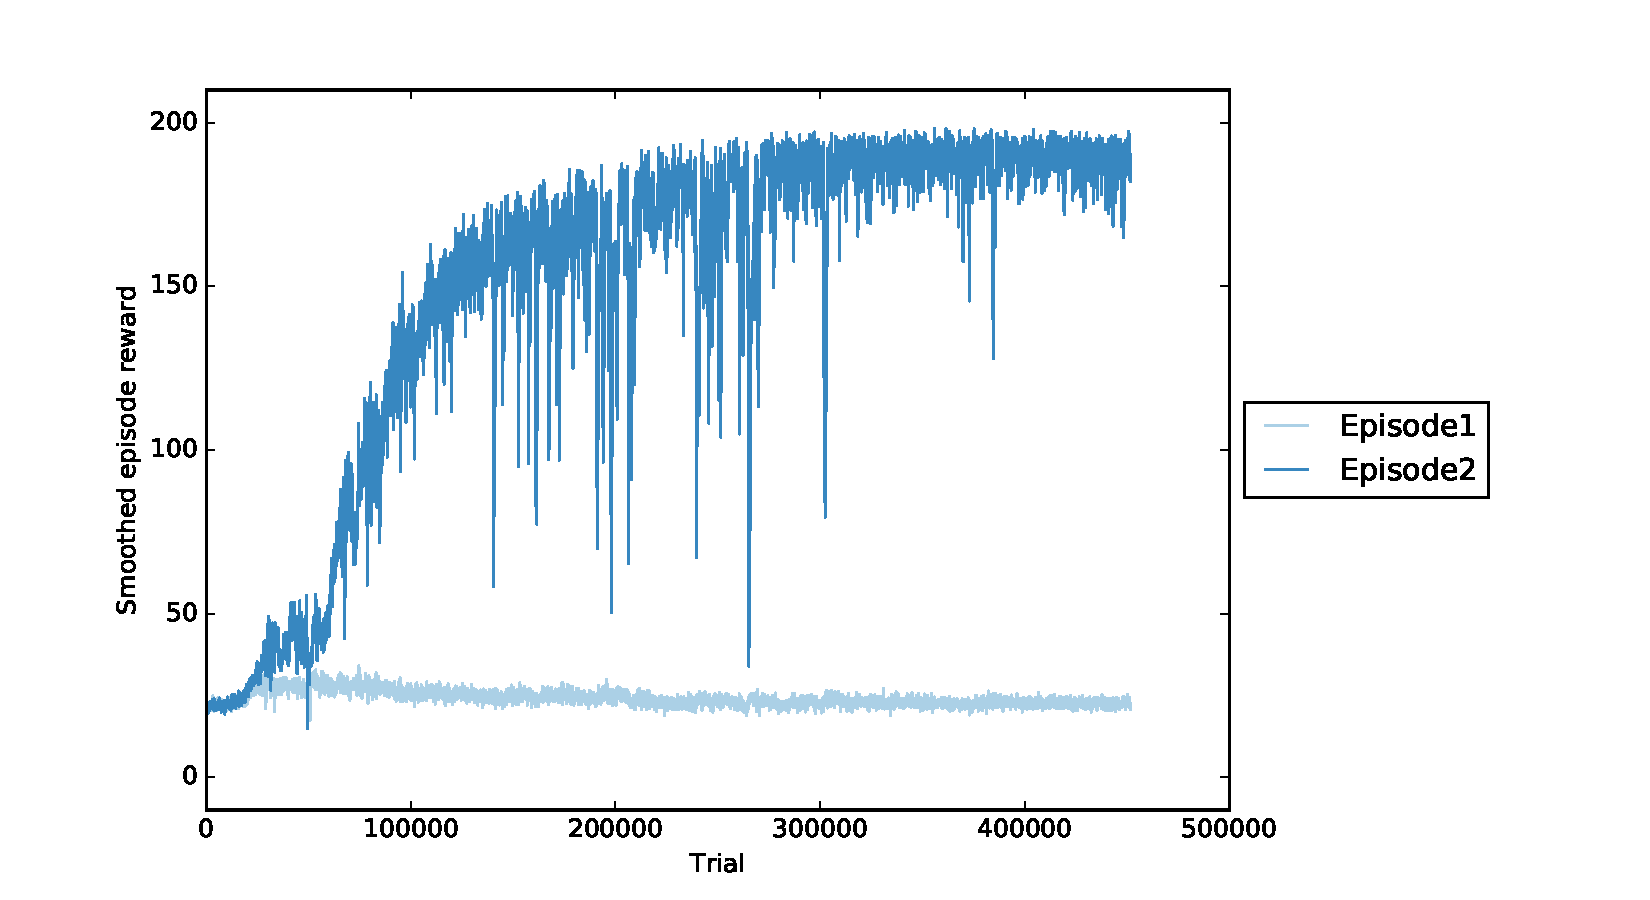
\includegraphics[width=0.49\linewidth]{fig/20permsLR2ep_training.pdf}}
	\\
	\subfloat[][Training over 5 episodes]{
		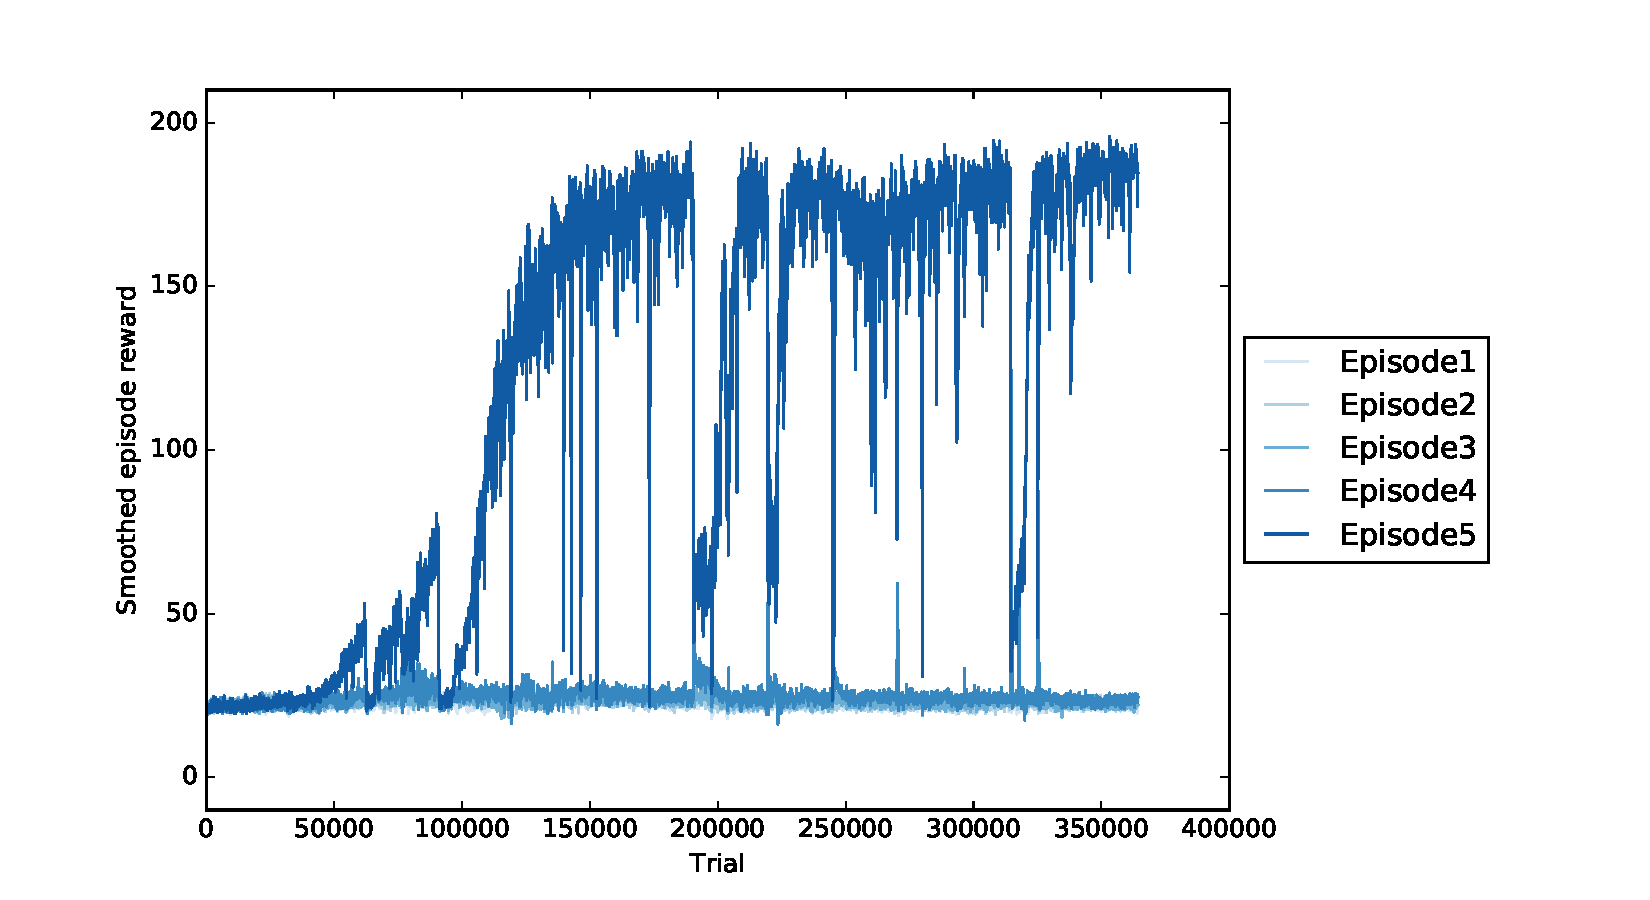
\includegraphics[width=0.9\linewidth]{fig/20permsLR5ep_training.pdf}}
	\caption{Episode-wise reward evolution when training on trials of 
	different lenghts}
	\label{fig:20permsLR_training}
\end{figure}

\begin{figure}
	\centering
	\subfloat[][2 episodes]{
		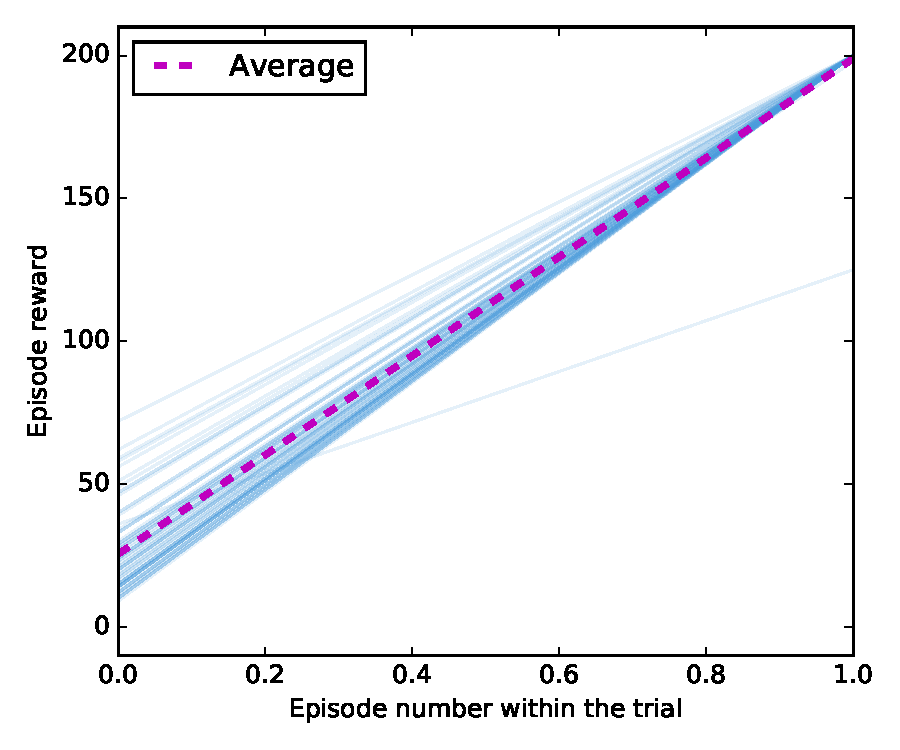
\includegraphics[width=0.33\linewidth]{fig/20permsLR2ep_rewards.pdf}}
	\subfloat[][5 episodes]{
		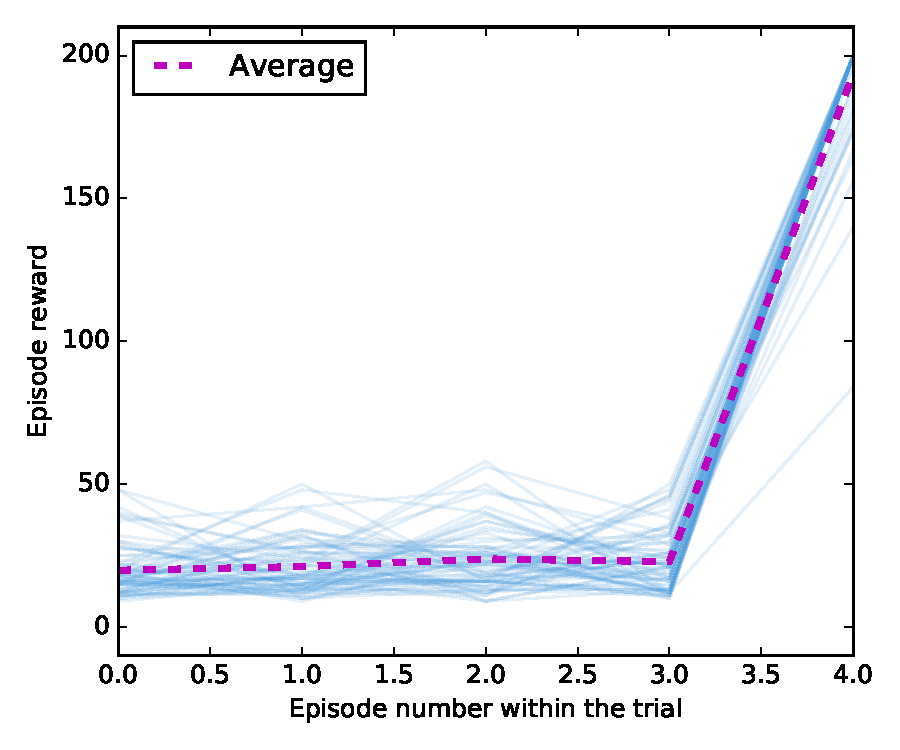
\includegraphics[width=0.33\linewidth]{fig/20permsLR5ep_rewards.pdf}}
	\subfloat[][10 episodes]{
		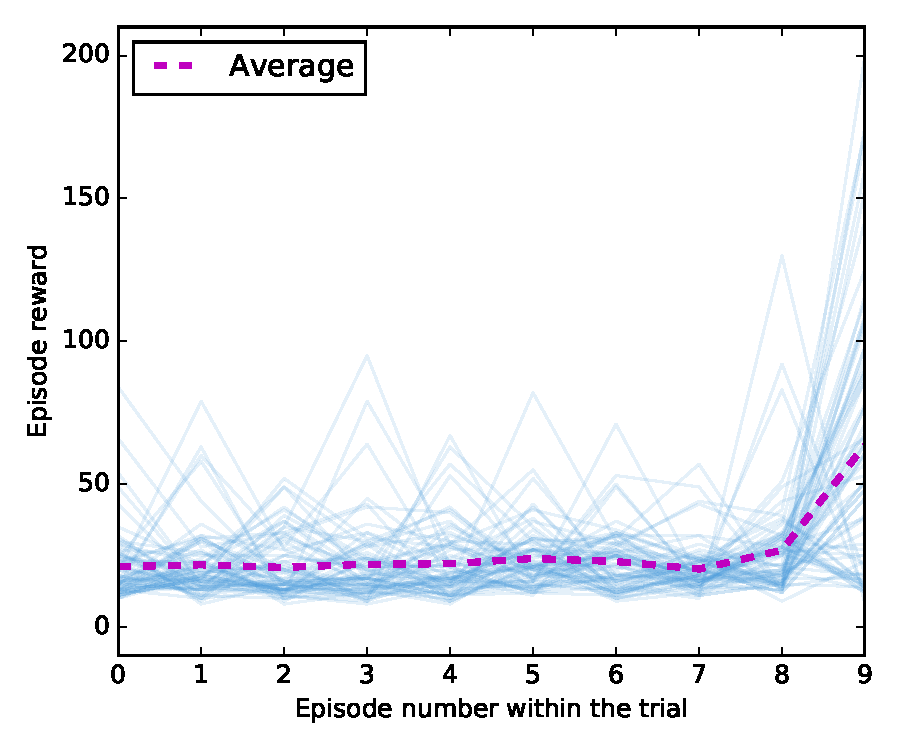
\includegraphics[width=0.33\linewidth]{fig/20permsLR10ep_rewards.pdf}}
	\caption{Testing performance of agents trained on trials of different
	lenghts. Several runs are displayed in blue on the same plot, and their
	average is shown as a red dashed line.}
	\label{fig:20permsLR_rewards}
\end{figure}

\begin{figure}
	\centering
	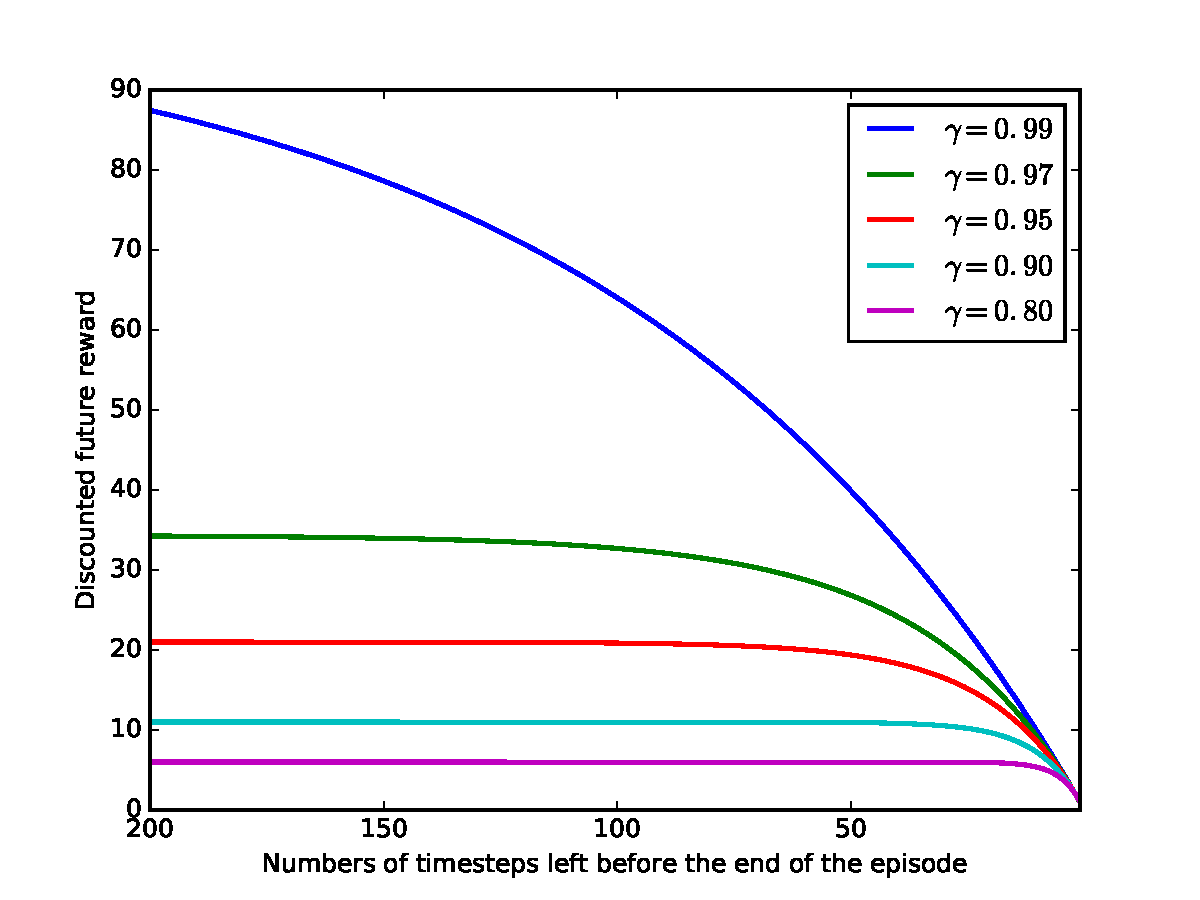
\includegraphics[width=0.8\linewidth]{fig/gamma_impact.pdf}
	\caption{Value of the discounted expected reward $R_t$ as a function
	of the number of timesteps left before the end of an episode in which
	a reward of +1 is given at every timestep; shown for different values
	of $\gamma$.}
	\label{fig:gamma_impact}
\end{figure}

\section{Problems with a 1-per-timestep reward}
This behaviour is linked to the dynamics of the expected future reward, 
the chosen discount factor and the reward structure of the environment.
In our case, the environment gives a constant +1 reward at every timestep of
a CartPole episode. If we choose a discount factor $\gamma=0.9$, the
discounted future reward at timesteps which are more than 50 timesteps away
from the end of the episode will be almost exactly equal (see 
Figure~\ref{fig:gamma_impact}).\\

This means that if an action that defines whether the episode ends or continues
at time $t$ has to be taken before time $t-50$, there is no way to link the
end of the episode with the action that was wrongly taken. This can be turned
around to say that actions do not really matter as long as the end of the
constant reward stream is more than 50 timesteps away for $\gamma=0.9$. In
our case, this explains why all episodes prior to the last one achieve low
reward. Because in every case, if the last episode is longer than 50
timesteps, the end of the reward stream is too far for the second-to-last 
episode to take it into account (if $\gamma=0.9$).\\

This should make the reader wonder why the last episode lasts 200 ticks;

\todo{why episode longer than 200 works?}


\section{Tuning the discount factor}
If we want to enforce good performance for non-terminal episodes, selecting
higher values for the discount factor is the first solution that comes to mind.
Unfortunately, besides the fact that this only enforces $k$ last episodes
to have a high reward (instead of trying to maximise performance as soon as
possible), this solution doesn't seem to work, as Figure~\ref{fig:varied_gamma}
shows.\\

In this experiment, we selected 3 training permutations (see 
Table~\ref{tab:5perms}) and trained our agent for 5 episodes. Several trainings
were run with different values for the discount factor $\gamma$.\\

\begin{table}
	\centering
	\caption{State permutations used for training}
	\label{tab:5perms}
	\bgroup
	\def\arraystretch{1.5}
	\begin{tabular}{c|c|c}
		[0, 1, 2, 3] & [0, 1, 3, 2] & [1, 0, 2, 3] \\
	\end{tabular}
	\egroup
\end{table}

Even though the rewards of previous episodes clearly climb higher as
we increase the discount factor, they all eventually decline to random
policy-like reward. Once the discount factor reaches values where the
second-to-last episode should be involved in having a high reward (around
0.97 and above), training diverges and the agent never manages to reach
high scores.\\

\begin{figure}
	\centering
	\subfloat[][$\gamma=0.82$]{
		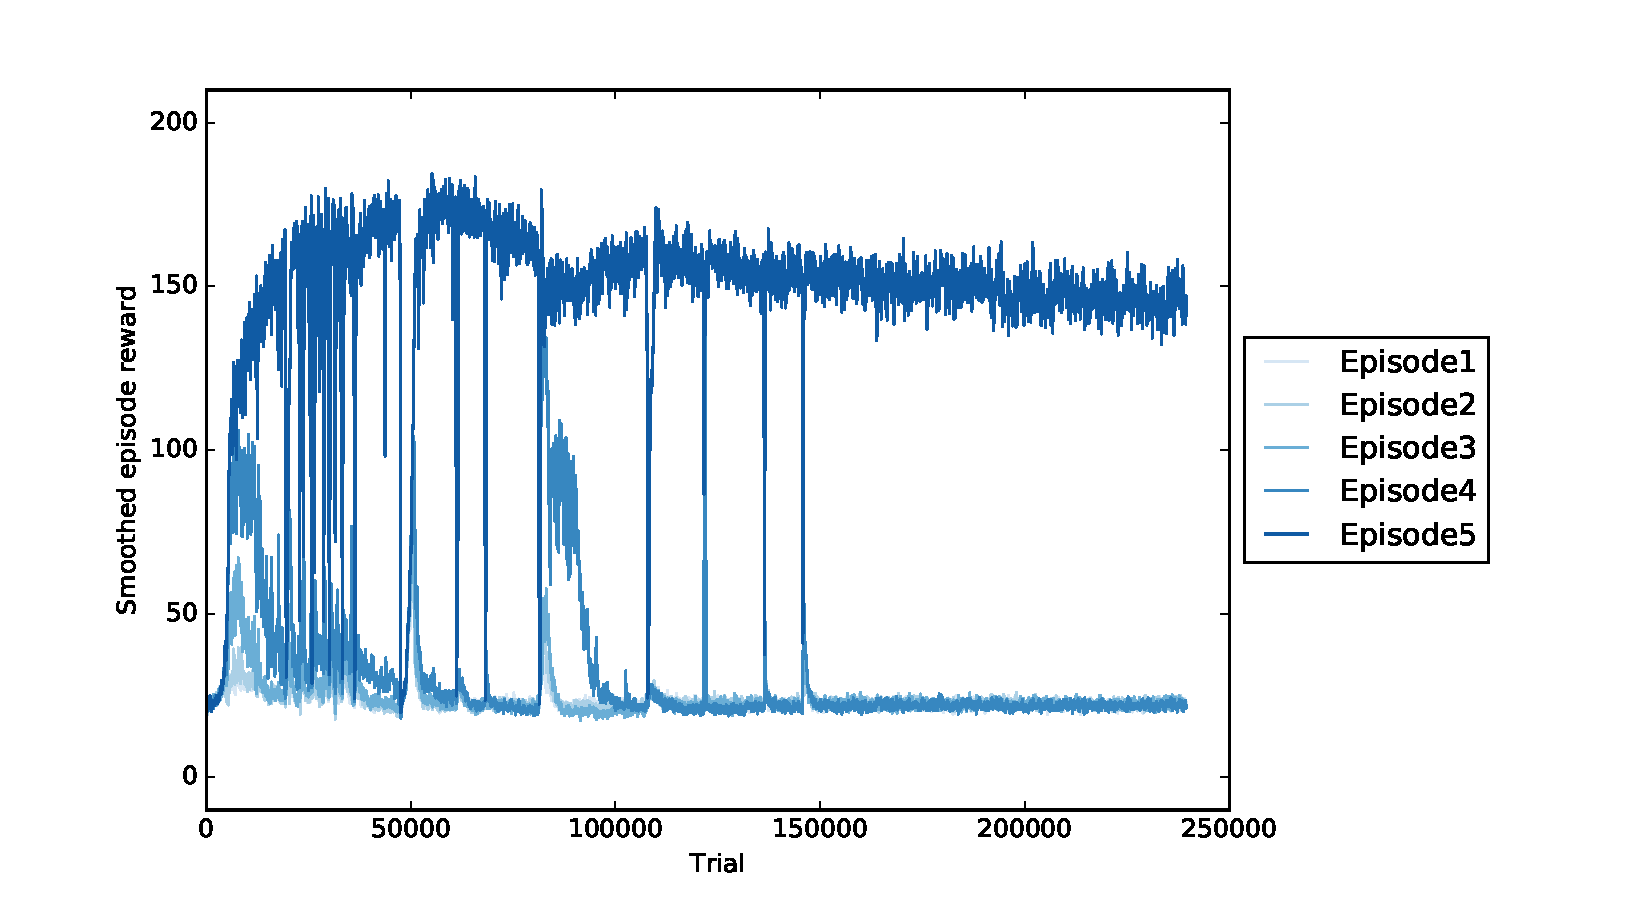
\includegraphics[width=0.49\linewidth]{fig/res_perms5ep_82.pdf}}
	\subfloat[][$\gamma=0.85$]{
		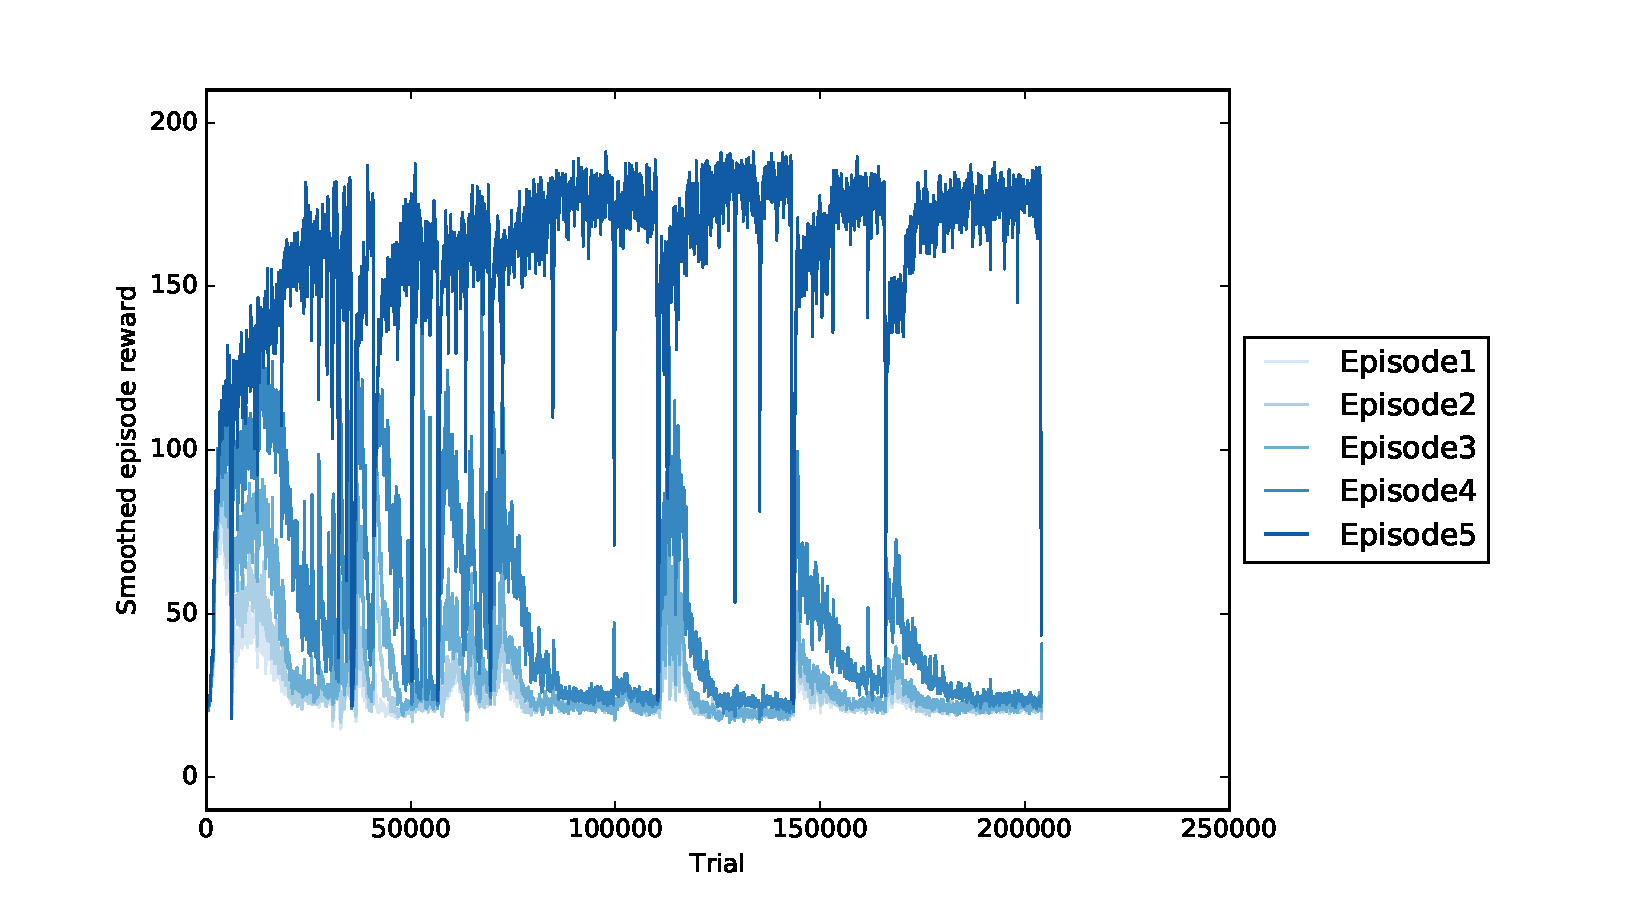
\includegraphics[width=0.49\linewidth]{fig/res_perms5ep_85.pdf}}
	\\
	\subfloat[][$\gamma=0.88$]{
		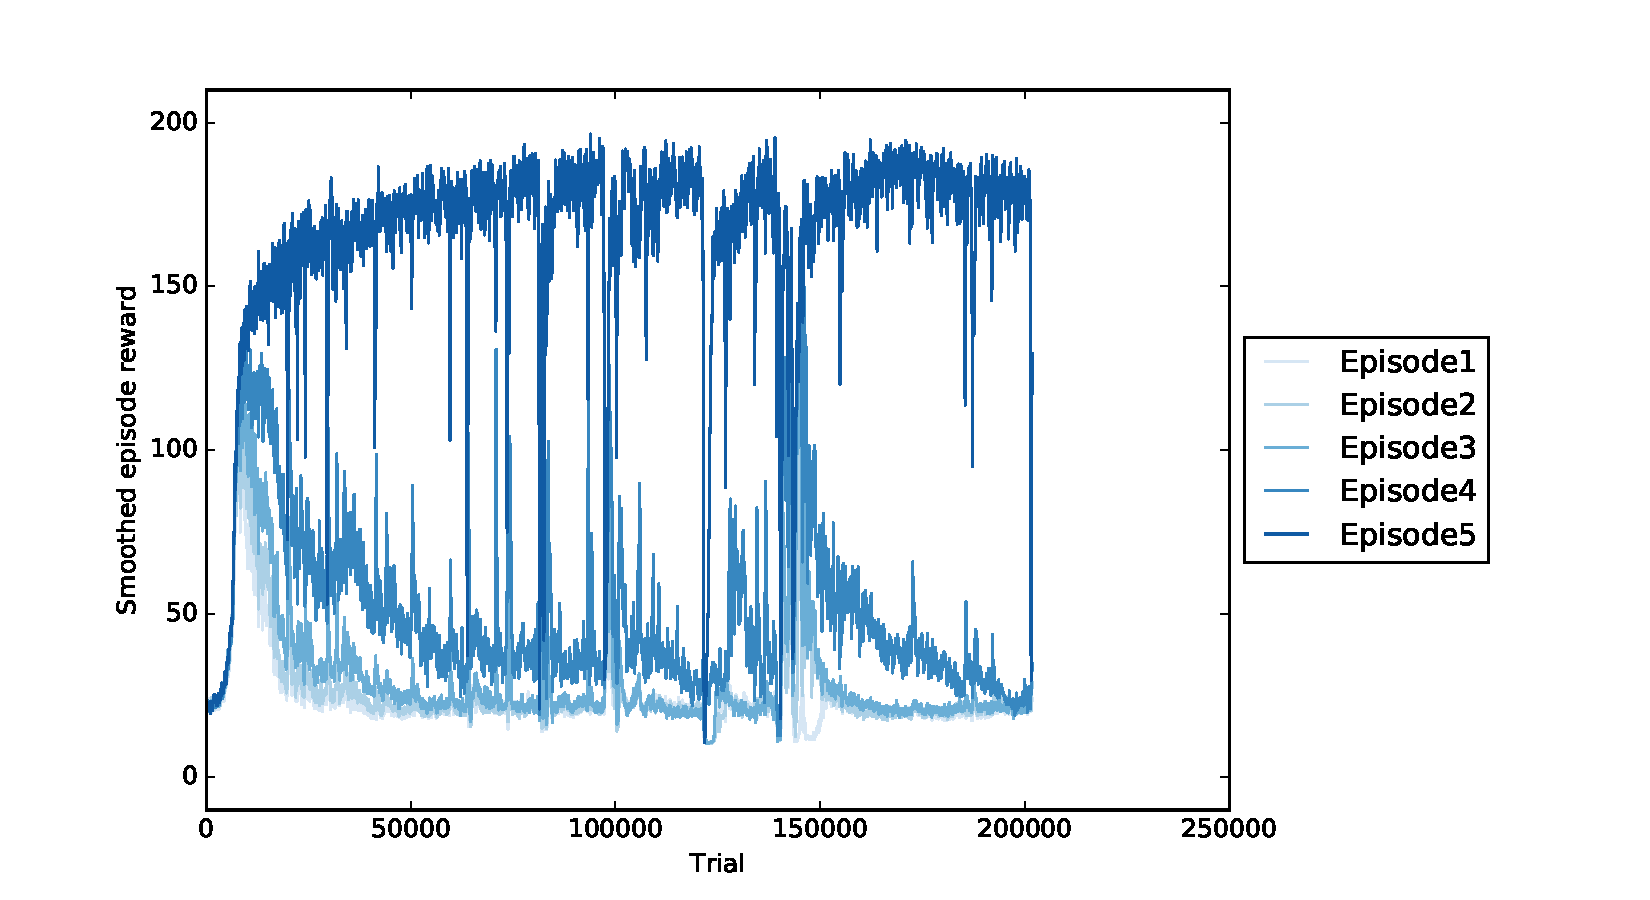
\includegraphics[width=0.49\linewidth]{fig/res_perms5ep_88.pdf}}
	\subfloat[][$\gamma=0.91$]{
		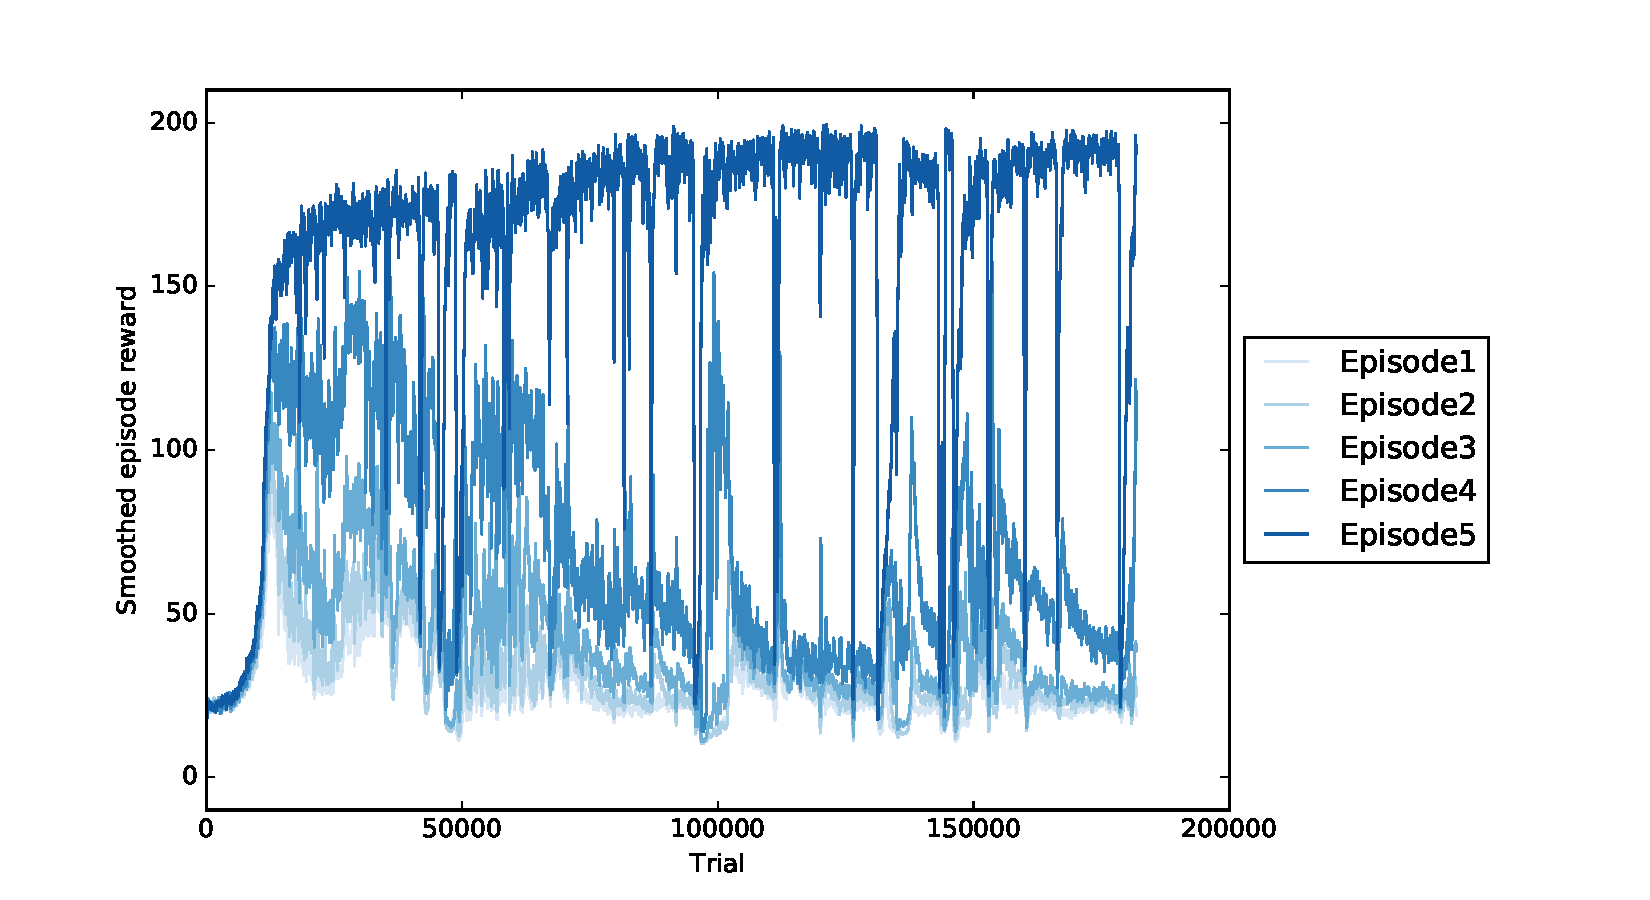
\includegraphics[width=0.49\linewidth]{fig/res_perms5ep_91.pdf}}
	\\
	\subfloat[][$\gamma=0.94$]{
		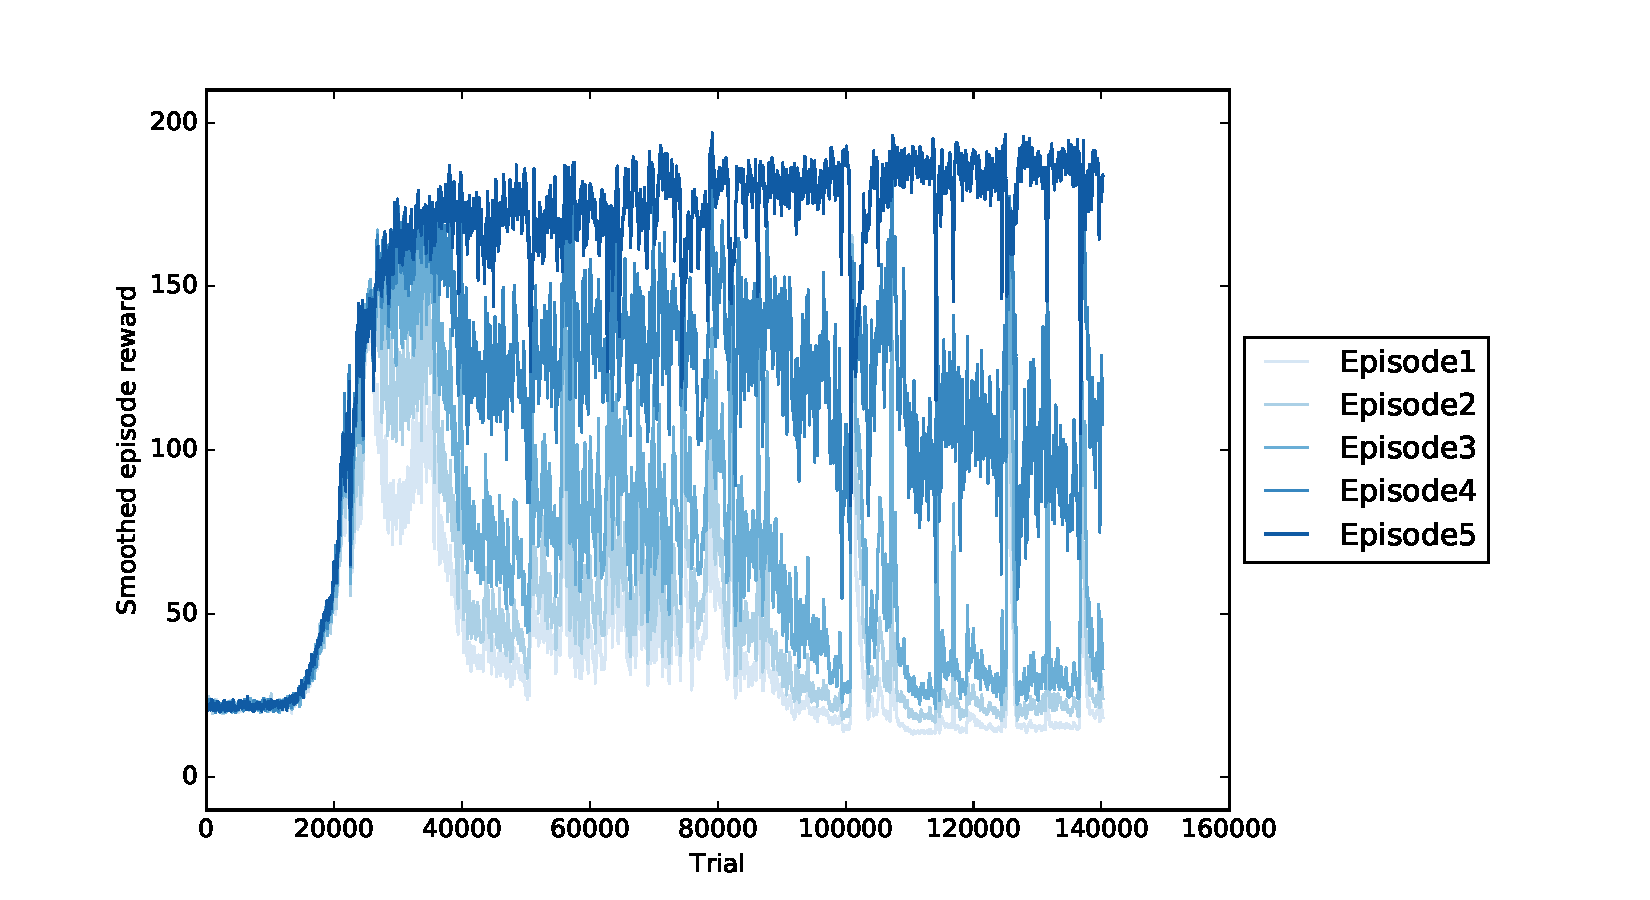
\includegraphics[width=0.49\linewidth]{fig/res_perms5ep_94.pdf}}
	\subfloat[][$\gamma=0.97$]{
		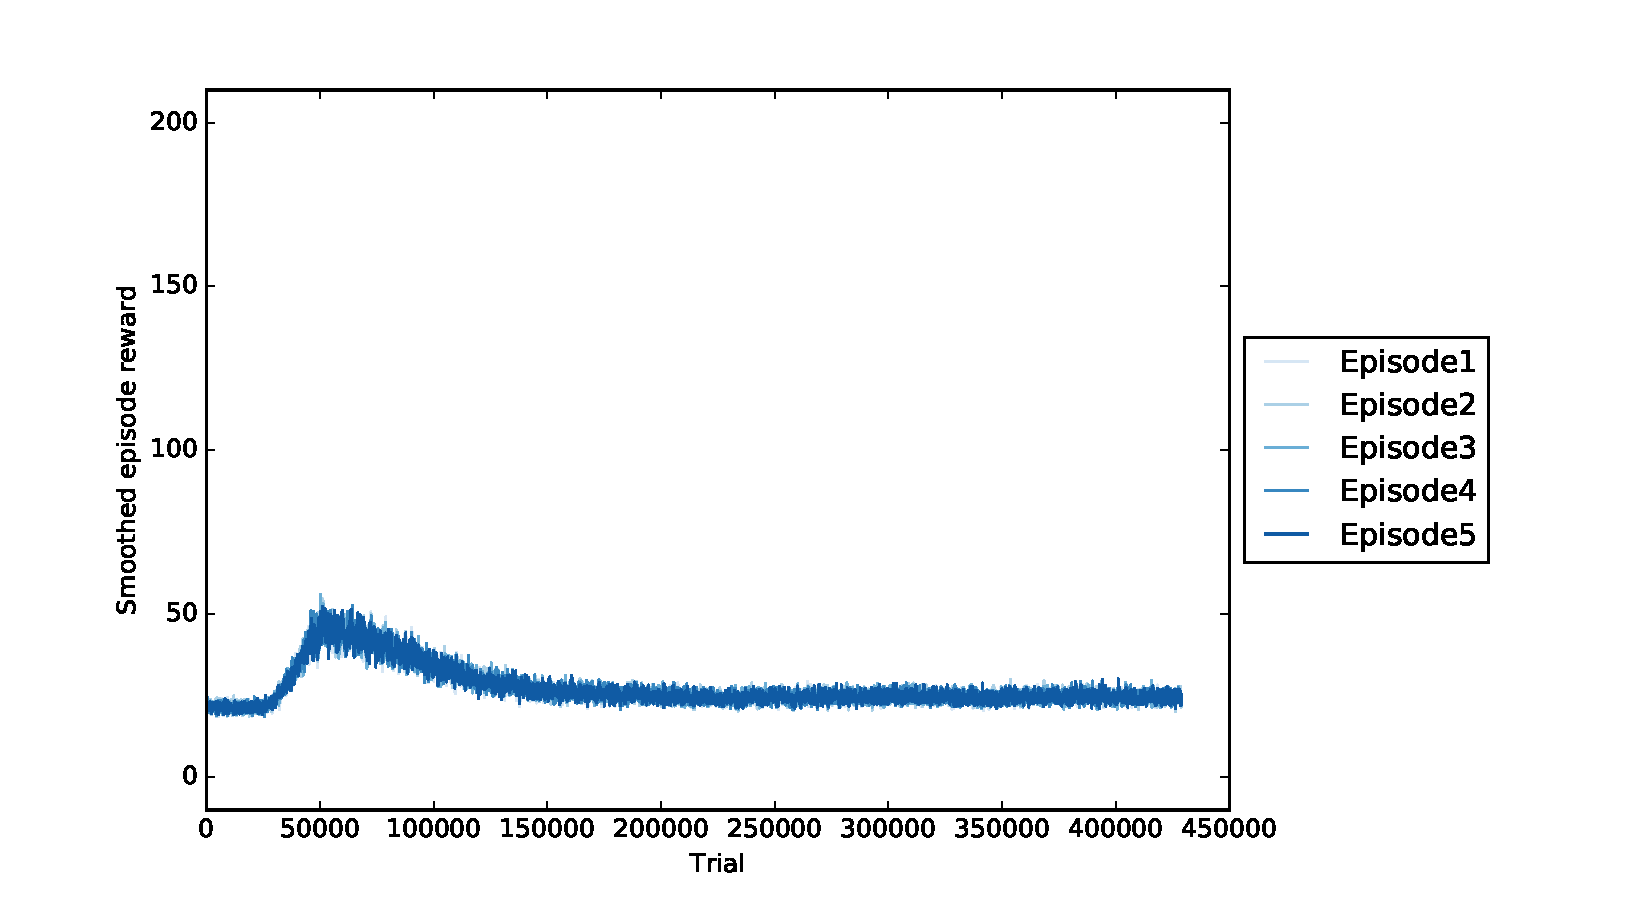
\includegraphics[width=0.49\linewidth]{fig/res_perms5ep_97.pdf}}
	\\
	\caption{Variation of the episode-wise reward evolution in trials of 5
	episodes when tuning the discount factor $\gamma$.}
	\label{fig:varied_gamma}
\end{figure}

\todo{how do we discuss and explain?}
\todo{also, if it learns to balance from the state, when it gets the same
state in prior episodes, why doesn't it do the same thing?}
